% "The trace is the position": a role's state is not stored — it is RECOMPUTED by
% replaying the recorded events through the projection functor. The stored global_type
% plus the event log fully determine every role's (state, stack). Palette: contract=indigo,
% events=slate, replay=teal, position=teal, accept=green.
\documentclass[border=10pt]{standalone}
\usepackage{tikz}
\usepackage{amsmath}
\usepackage{xcolor}
\usetikzlibrary{arrows.meta, positioning, fit, backgrounds}
\definecolor{contract}{HTML}{3730A3}
\definecolor{ev}{HTML}{475569}
\definecolor{rep}{HTML}{0D9488}
\definecolor{good}{HTML}{16A34A}
\definecolor{ink}{HTML}{1E293B}
\begin{document}
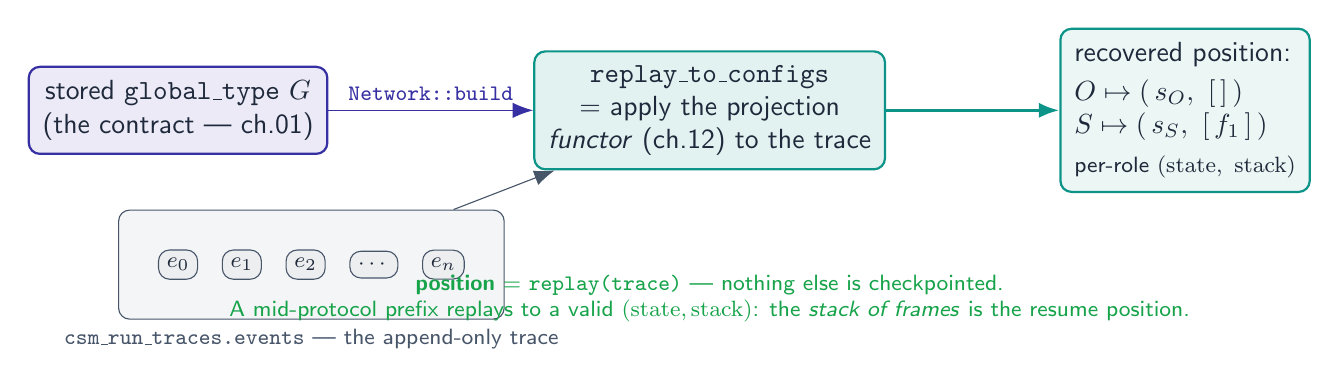
\begin{tikzpicture}[font=\sffamily, >={Latex[length=2.6mm]}, node distance=7mm,
    box/.style={draw, thick, rounded corners, align=center, inner sep=5pt, text=ink},
    ev/.style={draw=ev, fill=ev!10, rounded corners, inner sep=3pt, font=\sffamily\footnotesize, text=ink}]

  % stored contract
  \node[box, draw=contract, fill=contract!10] (g) {stored \texttt{global\_type} $G$\\(the contract — ch.01)};

  % event log
  \node[ev, below=12mm of g] (e0) {$e_0$};
  \node[ev, right=3mm of e0] (e1) {$e_1$};
  \node[ev, right=3mm of e1] (e2) {$e_2$};
  \node[ev, right=3mm of e2] (e3) {$\cdots$};
  \node[ev, right=3mm of e3] (en) {$e_n$};
  \begin{scope}[on background layer]
    \node[draw=ev, fill=ev!6, rounded corners, fit=(e0)(en), inner sep=5mm,
          label={[text=ev, font=\sffamily\footnotesize]below:\texttt{csm\_run\_traces.events} — the append-only trace}] (log) {};
  \end{scope}

  % replay engine
  \node[box, draw=rep, fill=rep!12, right=26mm of g] (rep)
    {\texttt{replay\_to\_configs}\\$=$ apply the projection\\\emph{functor} (ch.12) to the trace};

  % recovered positions
  \node[box, draw=rep, fill=rep!8, right=22mm of rep, align=left] (pos)
    {recovered position:\\[2pt]
     $O \mapsto (\,s_O,\ [\,]\,)$\\
     $S \mapsto (\,s_S,\ [\,f_1\,]\,)$\\[2pt]
     {\footnotesize per-role $(\mathrm{state},\ \mathrm{stack})$}};

  \draw[->, contract] (g) -- node[above, font=\sffamily\footnotesize]{\texttt{Network::build}} (rep);
  \draw[->, ev] (log) -- (rep);
  \draw[->, rep, very thick] (rep) -- (pos);

  \node[good, font=\sffamily\footnotesize, align=center, below=12mm of rep]
    {\textbf{position} $=$ \texttt{replay(trace)} — nothing else is checkpointed.\\
     A mid-protocol prefix replays to a valid $(\mathrm{state},\mathrm{stack})$: the \emph{stack of frames} is the resume position.};
\end{tikzpicture}
\end{document}
